\documentclass{article}

\usepackage{arxiv}

\usepackage[utf8]{inputenc}
\usepackage[T1]{fontenc}
\usepackage[numbers]{natbib}
\usepackage{hyperref}
\usepackage{xurl}
\usepackage{booktabs}
\usepackage{amsfonts}
\usepackage{nicefrac}
\usepackage{microtype}
\usepackage{amsmath}
\usepackage{graphicx}

\title{Decodability and Causal Control of Epistemic Uncertainty in LLMs}
\author{
    Feifan Liu \\
    The University of Texas at Austin \\
    \texttt{feifan.liu@utexas.edu} \\
    \And
    Amin Alipour \\
    University of Houston \\
    \texttt{maalipou@central.uh.edu} \\
}
\date{August 2026}

\begin{document}
\maketitle

\begin{abstract}

    Large Language Models (LLMs), in part due to being rewarded for overconfidence during post-training, frequently hallucinate and confidently assert falsehoods. Recent work has used interpretability techniques to show that an LLM's uncertainty in its response can be decoded from its activations. We study the properties of model uncertainty across four model families (Gemma-2, Qwen2.5, Llama-3.1, and GPT-2) and answer two questions: first, whether a direction encoding uncertainty can be decoded from activations, and second, whether that decoded direction causally affects the model's expressed confidence. We present the following four findings. First, uncertainty can be decoded as a linear direction in every model with 7B parameters or more (transfer accuracy $0.78$--$0.92$). This direction is present after pre-training, though instruction tuning sharpens it further: under a selection-free estimator, probes on instruct checkpoints outperform their base counterparts by $0.02$--$0.08$. Second, the existence of a decodable uncertainty direction does not imply the ability to causally steer the model: across model families, steering behavior and efficacy vary greatly. Third, a decoded direction that is ineffective when injected at a single site can become effective when injected across a band of layers. Fourth, the uncertainty direction decoded from one family does not transfer to another.

\end{abstract}

\section{Introduction}

Large Language Models (LLMs) are increasingly embedded in daily activities, businesses, and core economic functions. As of 2026, about half of U.S. adults report using AI chatbots, and 44\% have used ChatGPT~\citep{pew2026ai}. Despite their utility, LLMs are known to frequently hallucinate facts and confidently output misleading or incorrect statements. Previous work has identified a likely root cause: reinforcement learning from human feedback (RLHF) may introduce sycophantic tendencies in LLMs, as models learn human preferences~\citep{sharma2023sycophancy}. RLHF tends to reward LLMs for confident statements, much like it rewards the length of an answer or the model's perceived helpfulness.

LLM hallucinations and overconfidence pose a real threat, especially as model capabilities diffuse. This problem motivates the research area of model calibration or uncertainty quantification. We would like to elicit calibrated model answers that reflect the model's genuine internal confidence in its answer. We define model uncertainty as this internal confidence.

Previous work has shown that interpretability techniques, such as the use of linear probes, can extract directions in latent space that seem to encode model uncertainty. Recent work has observed that the best-detecting direction is not always the best steering direction~\citep{vonrutte2024guide}. However, previous work has yet to explore how this relationship between decodability and steerability behaves for epistemic uncertainty and how it might differ across base and instruct checkpoints.

Our work seeks to develop a better understanding of how models encode uncertainty, from the factors involved in whether a model has a decodable uncertainty direction to the properties of that direction and its ability to steer the model's behavior.

We study uncertainty across four model families: Gemma-2~\citep{gemma2024}, Qwen2.5~\citep{qwen2024}, Llama-3.1~\citep{llama2024}, and GPT-2~\citep{radford2019language}, and conduct experiments using linear probing and steering to study the properties of model uncertainty. After curating a dataset centered around a specific topic (the impact of artificial intelligence in education) and split across two axes -- time and certainty -- we extract uncertainty directions where possible and run experiments with steering.\footnote{All code, prompts, probe outputs, and steering result CSVs are available at \url{https://github.com/feifanl/llm-uncertainty-quantification}. Every number reported in this paper is regenerated from the committed CSVs by \texttt{viz/make\_paper\_tables.py}.}

Our contributions are:
\begin{enumerate}
    \item Every model we studied (except GPT-2) contains a decodable linear direction that corresponds to model uncertainty. Probe accuracy when transferring across the temporal axis ranges from 0.78 to 0.92, well above a bag-of-words control that collapses to chance on the same split. This direction is present after pre-training: base and instruct versions of the same model family decode at comparable accuracy. Instruct versions are modestly ahead ($0.02$--$0.08$) under a selection-free estimator.
    \item We introduce a controlled protocol for steering: an injection scale relative to the residual norm, a matched-norm random direction control, and a confidence metric using an LLM judge. We use this steering protocol to show that causal steerability does not always track decodability.
    \item We show that injecting a steering vector at a single site can be insufficient: in Qwen, a steering direction ineffective at one layer becomes causal when injected across multiple layers.
    \item We show that the uncertainty direction does not transfer across model families, even between models with identical residual width.
\end{enumerate}

\section{Related Work}

\textbf{Sycophancy and calibration.} Previous work has shown that RLHF-trained models tend to be sycophantic, preferring agreeable and pleasant responses to truthful ones~\citep{sharma2023sycophancy}. Other works study whether models are properly calibrated: \citet{kadavath2022know} show that models can often predict whether they know the answer to a question, and \citet{lin2022teaching} train models to express their uncertainty in words. These works measure and relate to \emph{expressed} calibration. In contrast, our research considers the properties of an \emph{internal} uncertainty signal in model activations.

\textbf{Probing and linear representations.} Previous interpretability work has shown that high-level traits and concepts such as truthfulness can often be linearly decoded from residual-stream activations~\citep{azaria2023internal, burns2022discovering, marks2023geometry}. These prior findings are consistent with the linear representation hypothesis~\citep{park2023linear}. \citet{ahdritz2024distinguishing} investigate epistemic versus aleatoric uncertainty and find that the uncertainty signal transfers across domains. However, decodability does not necessarily imply that a direction is used by the model and thus causally steerable. Control-task and amnesic probe studies have shown that a probe can successfully decode information that the model does not depend on for its behavior~\citep{hewitt2019designing, elazar2021amnesic}. This motivates our causal tests. We add activation steering, a dataset that controls for time as a confounding variable, and a cross-model-family comparison to~\citet{ahdritz2024distinguishing}.

\textbf{Activation steering and ablation.} Adding or removing a direction from the residual stream during model generation is an established causal test for a decoded representation~\citep{turner2023activation, panickssery2023caa, zou2023representation}. For example,~\citet{arditi2024refusal} show that model refusal is mediated by a single difference-of-means direction. \citet{li2023iti} train probes to detect truthfulness and then steer activations using the decoded direction at inference time. We apply the same pattern to epistemic uncertainty. \citet{vonrutte2024guide} guide high-level concepts such as truthfulness, appropriateness, and quality, observing that probes that find a direction with the best detection accuracy are not always the best at steering. \citet{galeone2026perfect} report a similar detection--control gap for hallucination. We extend this line of research to epistemic uncertainty. We improve upon the standard single-site steering protocol with a relative-norm injection scale, a matched-norm random control, a multi-layer band injection, and a cross-model-family transfer test. This protocol allows us to distinguish a legitimate causal effect from generic disruptions.

\section{Methods}

\subsection{Models}

We study four model families, listed in Table~\ref{tab:models}. For the base vs.\ instruct comparison (Section~\ref{sec:decode}), we use both the pretrained (base) and instruct checkpoints of each family. Since GPT-2 does not have an instruct checkpoint, we omit its base vs.\ instruct comparison. All models run in \texttt{bfloat16} with greedy decoding.

\begin{table}[h]
    \centering
    \begin{tabular}{llc}
        \toprule
        Family & Checkpoints (base / instruct) & Params \\
        \midrule
        Gemma-2-9b    & \texttt{google/gemma-2-9b} / \texttt{-it}                    & 9.2B \\
        Qwen2.5-7B    & \texttt{Qwen/Qwen2.5-7B} / \texttt{-Instruct}               & 7.6B \\
        Llama-3.1-8B  & \texttt{meta-llama/Llama-3.1-8B} / \texttt{-Instruct}       & 8.0B \\
        GPT-2-large   & \texttt{gpt2-large} (base only)                             & 0.77B \\
        \bottomrule
    \end{tabular}
    \caption{Model checkpoints. We use Gemma-2-9b and Qwen2.5-7B for the cross-model-family transfer control (Section~\ref{sec:transfer}), since they both share a residual width of $3584$.}
    \label{tab:models}
\end{table}

\subsection{Dataset and prompt design}

We construct a dataset of 100 items related to the impact of artificial intelligence in education. Each item is a claim with a known/unknown label and five paraphrases that preserve semantic meaning. Each item follows the template

\texttt{Q: Is the following claim true? "\{claim\}"\textbackslash nA:}

The dataset is split evenly across two crossed axes: a known/unknown label axis and a past/future temporal axis. This gives us 50 past and 50 future items, where each half is split into 25 known and 25 unknown (25 items per cell). The temporal axis allows us to control for time as a confounding variable. Without the axis, a linear probe could naively classify known/unknown prompts using temporal features alone, such as classifying all future prompts as unknown. We also eliminate evidential phrases from the dataset (e.g.\ ``research shows,'' ``empirically''), since a simple bag-of-words probe scores above random chance using these phrases as heuristics.

For causal experiments, we use a held-out dataset of 40 neutral out-of-distribution prompts including facts, explanatory questions, procedures, and open questions. We constructed the held-out dataset using a variety of topics in order to isolate steering effects from the training topic of the probe.

\subsection{Linear probes and the transfer test}

We cache residual-stream activations at the last five prompt-token positions, written $p_0$ (fifth-from-last) through $p_4$ (final prompt token), and train a logistic-regression probe at every (layer, position) cell to classify the associated prompt as known vs.\ unknown. GPT-2-large is cached at one position only. Our primary metric is transfer accuracy: a probe's performance when trained on past items and then tested on future items (and vice versa, denoted p2f and f2p). We focus primarily on transfer performance, since the probe cannot simply memorize temporal markers (``past unknown and known prompts have these distinguishing characteristics''); thus, transfer accuracy more directly reflects model uncertainty. Test sets are balanced ($150$ known / $150$ unknown per direction) so that the accuracy of the probe at the threshold of $0.5$ is interpretable. We report accuracy rather than the area under the receiver operating characteristic curve (AUROC), since our probes already output hard yes/no responses. We report the peak transfer accuracy over layers and cached positions, so reported values are an upper bound rather than a point estimate on decodability. Table~\ref{tab:probe} also reports a stricter number than peak accuracy: we pick the cell using one transfer direction and score it on the other (Section~\ref{sec:limitations}). Probes are $\ell_2$-regularized logistic regressions ($\lambda = 10^{-3}$). We fit them via full-batch gradient descent on standardized activations. p2f trains on all $300$ past-axis prompts ($50$ items $\times$ $6$ text variants) and tests on the $300$ future-axis prompts; f2p does the reverse.

A TF-IDF bag-of-words classifier on raw prompts reaches $0.97$ but collapses to random chance when tested on the transfer split ($0.51$ p2f, $0.55$ f2p). This confirms that the transfer test removed surface signals that probes could otherwise naively exploit.

\subsection{Steering vector and relative scale}

The steering vector is the difference-of-means direction at a specific layer and the final token position,
\[
    v = \operatorname{mean}(h \mid \text{known}) - \operatorname{mean}(h \mid \text{unknown}),
\]
computed from the same activations. We inject $v$ by adding it to the residual stream of the chosen decoder layer at every position and every decoding step, scaled by $\alpha$. We use greedy decoding to attribute changes in outputs to steering rather than sampling noise.

Because the magnitude of the residual stream varies widely across models (mean $\lVert h \rVert \approx 276$ in Gemma-2-9b vs.\ $\approx 82$ in Qwen2.5-7B), we normalize $\alpha$ to a relative scale. We do this by scaling $v$ to its unit vector and multiplying it by the mean residual norm of the chosen layer, so that $\alpha$ represents a fraction of the residual magnitude. The relative $\alpha$ scale avoids over- and under-steering, allowing us to better compare steering efficacy across model families. We steer across $\alpha \in \{-1, -0.5, -0.25, 0, 0.25, 0.5, 1\}$ and generate up to $80$ new tokens per prompt. For single-site steering, we inject $v$ at a fixed mid-stack layer chosen a priori (Gemma-2-9b layer $20$, Qwen2.5-7B layer $19$, Llama-3.1-8B layer $18$, GPT-2-large layer $22$). For Gemma and Qwen, the chosen layer falls within two layers of the probe's peak accuracy, while for Llama (peak layer $22$) and GPT-2 (peak layer $35$), it does not (Section~\ref{sec:limitations}). We set a coherent $\alpha$ range $[-0.5, 0.5]$: beyond this range, a large $|\alpha|$ creates incoherent or repetitive outputs regardless of the direction injected, so we do not treat an effect visible only at $|\alpha| = 1$ as evidence of steering. We consider a direction \emph{causal} when judge confidence increases monotonically with $\alpha$ inside the coherent range and the effect becomes distinguishable from the matched-norm random control, and \emph{inert} otherwise.

\subsection{Controls}

\textbf{Random-direction control.} To distinguish a decoded uncertainty direction from any random perturbation that is sufficiently large, we also inject a random Gaussian vector. The random-direction control is averaged over three seeds and has the same norm and scale as $v$.

\textbf{Cross-family transfer.} To test whether a decoded uncertainty direction transfers across model families, we inject a decoded direction from one model into another. A raw activation vector is only meaningful between models with equal residual width, so we only test this control on Gemma-2-9b and Qwen2.5-7B (both width $3584$).

\subsection{Confidence metric}
\label{sec:confidence}

We measure a model's expressed uncertainty and confidence via an instruct LLM judge~\citep{zheng2023judging} (Qwen2.5-7B-Instruct) on each model output. We query the judge via a forced Yes/No question (``Is the answer confident and assertive?''). We read confidence as $P(\text{Yes})/(P(\text{Yes})+P(\text{No}))$ from the next-token logits and scale it to the range $0$--$100$. Where noted, we re-score the same generations with a second, non-Qwen judge (Llama-3.1-8B-Instruct) to check that a result is not an artifact of one judge.

Rather than using a hand-tuned confidence metric, such as a counter for hedge-words that could easily break between model families that express uncertainty in different styles, we choose to use an LLM judge.

\subsection{Band injection}

Steering via single-site injection creates a diluted effect that is partially overwritten by downstream layers. In cases where single-site injection was ineffective, we test causal steerability by injecting a per-layer difference-of-means vector at every layer in a nine-layer band spanning the mid-to-late layer stack (Qwen2.5-7B layers $15$--$23$, Llama-3.1-8B layers $18$--$26$ and $20$--$28$). Because steering compounds across layers, we divide each layer's contribution by the band width (nine) to better compare multi-site injection to single-site.

\subsection{Base vs.\ instruct}

To test whether the decoded uncertainty representation is a result of RLHF or pre-training, we run the probe transfer test (p2f, f2p) on both the base and instruct versions of each model family.

\section{Results}

\subsection{Decodability is already present after pre-training}
\label{sec:decode}

Table~\ref{tab:probe} reports the peak transfer accuracy for base and instruct model checkpoints. In every model with 7B or more parameters, a probe can decode the uncertainty axis (known/unknown) well above random chance ($0.78$--$0.92$). Base and instruct checkpoints are similar, but instruct variants perform slightly better ($0.02$--$0.07$ under peak estimator, $0.02$--$0.08$ under selection-free estimator). The direction is already present after pre-training. The decoded difference-of-means directions in base and instruct variants are highly aligned (cosine $0.57$ for Llama and $0.75$ for Qwen versus $\approx 0.02$ for random same-width vectors). Instruction tuning appears to improve an existing direction rather than create a new one. Although GPT-2-large's probe scores near random chance ($0.55$), the model is small and old; thus, this result likely reflects a scale and capability floor rather than evidence that decodability is a result of RLHF (which GPT-2-large lacks).

The instruct advantage is not robust to how the readout cell is chosen, and we do not want to overstate it. The peak estimator selects a token position as well as a layer, and it lands on a different position for base and instruct in all three families (Table~\ref{tab:probe}), so the $\Delta$ column compares two differently-selected cells. Restricted to the final prompt token $p_4$ for both checkpoints, the selection-free advantage survives and grows ($+0.070$ Gemma, $+0.052$ Qwen, $+0.090$ Llama), but the peak advantage shrinks to $-0.013$, $+0.040$ and $+0.000$ respectively, and peak deltas computed separately at each cached position range from $-0.097$ to $+0.163$ and change sign within every family. We therefore read the instruct effect as a real but small gain in how broadly the axis is available across the layer--position grid, not as a large gain at any one readout site.

\begin{table}[h]
    \centering
    \begin{tabular}{lccccc}
        \toprule
        & \multicolumn{3}{c}{Peak (layer, position, direction)} & \multicolumn{2}{c}{Selection-free} \\
        \cmidrule(lr){2-4}\cmidrule(lr){5-6}
        Family & Base & Instruct & $\Delta$ & Base & Instruct \\
        \midrule
        Gemma-2-9b     & 0.903 (L26, $p_4$) & 0.923 (L25, $p_2$) & $+0.020$ & 0.688 & 0.770 \\
        Qwen2.5-7B     & 0.783 (L20, $p_4$) & 0.850 (L19, $p_2$) & $+0.067$ & 0.752 & 0.772 \\
        Llama-3.1-8B   & 0.847 (L30, $p_1$) & 0.910 (L28, $p_2$) & $+0.063$ & 0.678 & 0.733 \\
        GPT-2-large    & 0.553 (L35, $p_0$) & --                 & --       & 0.470 & -- \\
        \midrule
        TF-IDF baseline & \multicolumn{5}{c}{0.507 (p2f) / 0.547 (f2p)} \\
        \bottomrule
    \end{tabular}
    \caption{Residual-stream transfer accuracy. ``Peak'' is the best of p2f/f2p over the (layer, position) grid, with the selected cell in parentheses; it combines best-of-layer, best-of-position and best-of-direction and thus represents an upper bound. Note that the selected position differs between base and instruct in every family, so the $\Delta$ column is not a position-matched comparison; Section~\ref{sec:decode} gives the matched figures. If two layers are tied at three decimal places (Gemma instruct L25/26, Qwen base L20/24), the lower layer is listed. ``Selection-free'' is a point estimate rather than an upper bound---we pick the cell on one transfer direction and report the other and average over both orders. Transfer accuracy is higher in instruct variants than their base counterparts for both peak and selection-free estimators. The TF-IDF row is a bag-of-words control on the raw prompts.}
    \label{tab:probe}
\end{table}

Figure~\ref{fig:transfer} shows the transfer accuracy as a function of normalized layer depth. Decodability increases in the early-to-middle layers, peaking in the mid-to-late layers for the three larger models. GPT-2-large never separates from chance. The base and instruct variants track each other through the whole layer stack.

\begin{figure}[h]
    \centering
    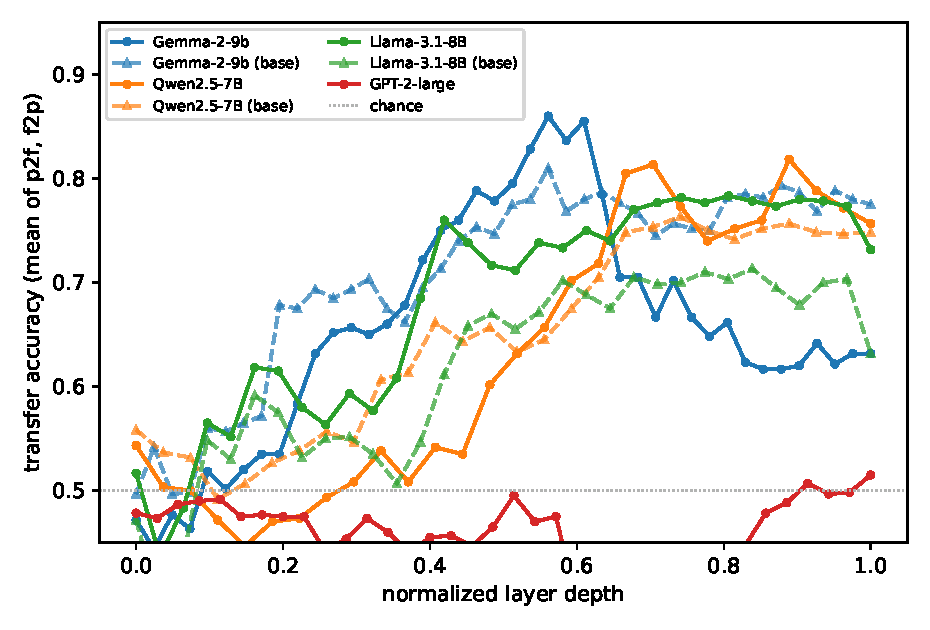
\includegraphics[width=0.7\linewidth]{figures/fig2_transfer_accuracy.pdf}
    \caption{Transfer accuracy vs.\ normalized layer depth. For each layer we average the p2f and f2p directions and then take the envelope over the cached token positions. Solid lines are instruct variants, dashed lines are the base counterpart. Depth is layer number divided by number of layers, so families with different layer depths share an axis. The dotted line marks chance ($0.5$). This figure averages the two transfer directions (p2f/f2p) while Table~\ref{tab:probe} picks the better one, so these curves are slightly below the table's peaks.}
    \label{fig:transfer}
\end{figure}

\subsection{Causal steerability does not track decodability}
\label{sec:steer_causal}

Table~\ref{tab:steer} summarizes the causal experiments in the instruct models. Most notably, the steerability of models does not track decodability and varies widely. Gemma is causally steerable via single-site injection, with judge confidence increasing monotonically from $30$ to $65$ across the coherent $\alpha$ band ($|\alpha| \le 0.5$), while the random control stays near $50$. Qwen fails when steered via single-site injection (own-direction $\approx$ random), but steering becomes causal when we use multi-site injection (confidence increases from $33$ to $57$ and separates cleanly from the random control). Llama fails when steering via single-site and multi-site injection at the chosen layer $18$, despite having a transfer accuracy ($0.80$) similar to that of Qwen. GPT-2, consistent with its near random chance probe performance and size, shows no legible effect.

Because Llama's probe peaks at layer $22$ rather than layer $18$, we reran both injection methods around layer $22$ (single-site at layer $22$, multi-site at layers $20$--$28$). Inside the coherent $\alpha$ range, the null holds: own-direction confidence at $\alpha = -0.5$ is $45.4$ versus $48.9$ for the matched random control, and both correlations remain indistinguishable from zero ($+0.03$ $[-0.08, +0.13]$ single-site, $+0.05$ $[-0.03, +0.14]$ multi-site; Table~\ref{tab:steer}). A large and asymmetric effect does appear, but only at $|\alpha| = 1$, outside of the coherent $\alpha$ range. Steering toward unknown under multi-site injection drives mean confidence down to $8.5$ while the matched random control stays near baseline ($50.7$), a gap both our primary judge and the second, non-Qwen judge agree on. Steering toward known produces no comparable separation.

We do not read this as a clean causal result. At $\alpha = -1$, $21$ of the $40$ own-direction generations degenerate into repetition, against $0$ of the $120$ control generations (three seeds $\times$ 40 prompts). The two means are computed over samples that are not comparable. Llama's decoded direction is inert inside the coherent $\alpha$ range, that is, wherever generation stays coherent.

Thus, steerability is not necessarily predicted by decodability. It varies by model family, injection site, and probe layer.

\begin{table}[h]
    \centering
    \begin{tabular}{llcccc}
        \toprule
        Model & Site & Accuracy$^\ddagger$ & Single-site & Band & corr$^\dagger_{\text{own}}$ (95\% CI) \\
        \midrule
        Gemma-2-9b-it         & L20              & 0.89 & causal ($30\!\to\!65$) & ---                    & $+0.25$ $[+0.14, +0.37]$ \\
        Qwen2.5-7B-Instruct   & L19 / L15--23    & 0.82 & inert                  & causal ($33\!\to\!57$) & $+0.20$ $[+0.08, +0.31]$ \\
        Llama-3.1-8B-Instruct & L18 / L18--26    & 0.80 & inert                  & inert                  & $+0.00$ $[-0.09, +0.09]$ \\
        Llama-3.1-8B-Instruct & L22 / L20--28    & 0.80 & inert                  & inert                  & $+0.05$ $[-0.03, +0.14]$ \\
        GPT-2-large           & L22              & 0.55 & inert                  & ---                    & $+0.10$ $[-0.02, +0.21]$ \\
        \bottomrule
    \end{tabular}
    \caption{Steering outcome by model over 40 prompts (random control over 3 seeds), scored by the primary judge. All rows are instruct checkpoints except GPT-2-large, which is base (it has no instruct release); its accuracy is the base probe value. The two Llama rows are the a priori site and the probe-peak site. $^\ddagger$Accuracy is the peak transfer accuracy over layers at the final prompt token $p_4$, best-of-direction; it is stricter than the corresponding Table~\ref{tab:probe} entry because it does not also select over token position. $^\dagger$corr is Pearson corr($\alpha$, confidence) over the coherent $\alpha$ band for the steering method reported on that row: single-site for Gemma and GPT-2, multi-site for Qwen and Llama. A 95\% confidence interval from $3000$ bootstrap resamples of the 40 prompts is reported: the CIs for the matched-norm random controls all include zero (Gemma $+0.02\,[-0.00,+0.05]$, Qwen $-0.02\,[-0.08,+0.04]$, Llama L18--26 $+0.03\,[-0.01,+0.08]$, Llama L20--28 $+0.01\,[-0.03,+0.05]$, GPT-2 $-0.05\,[-0.13,+0.02]$). Causal steerability does not track decodability: only Gemma and Qwen have own-direction CIs excluding both zero and their control, while Llama, which decodes as well as Qwen, is inert at both sites.}
    \label{tab:steer}
\end{table}

The dose-response curves in Figure~\ref{fig:steering} make the gradient visible. Only Gemma moves meaningfully at a single site---Qwen moves only under multi-site injection, Llama's own direction tracks its random control under both steering methods, and GPT-2 does not separate from its control at all.

\begin{figure}[h]
    \centering
    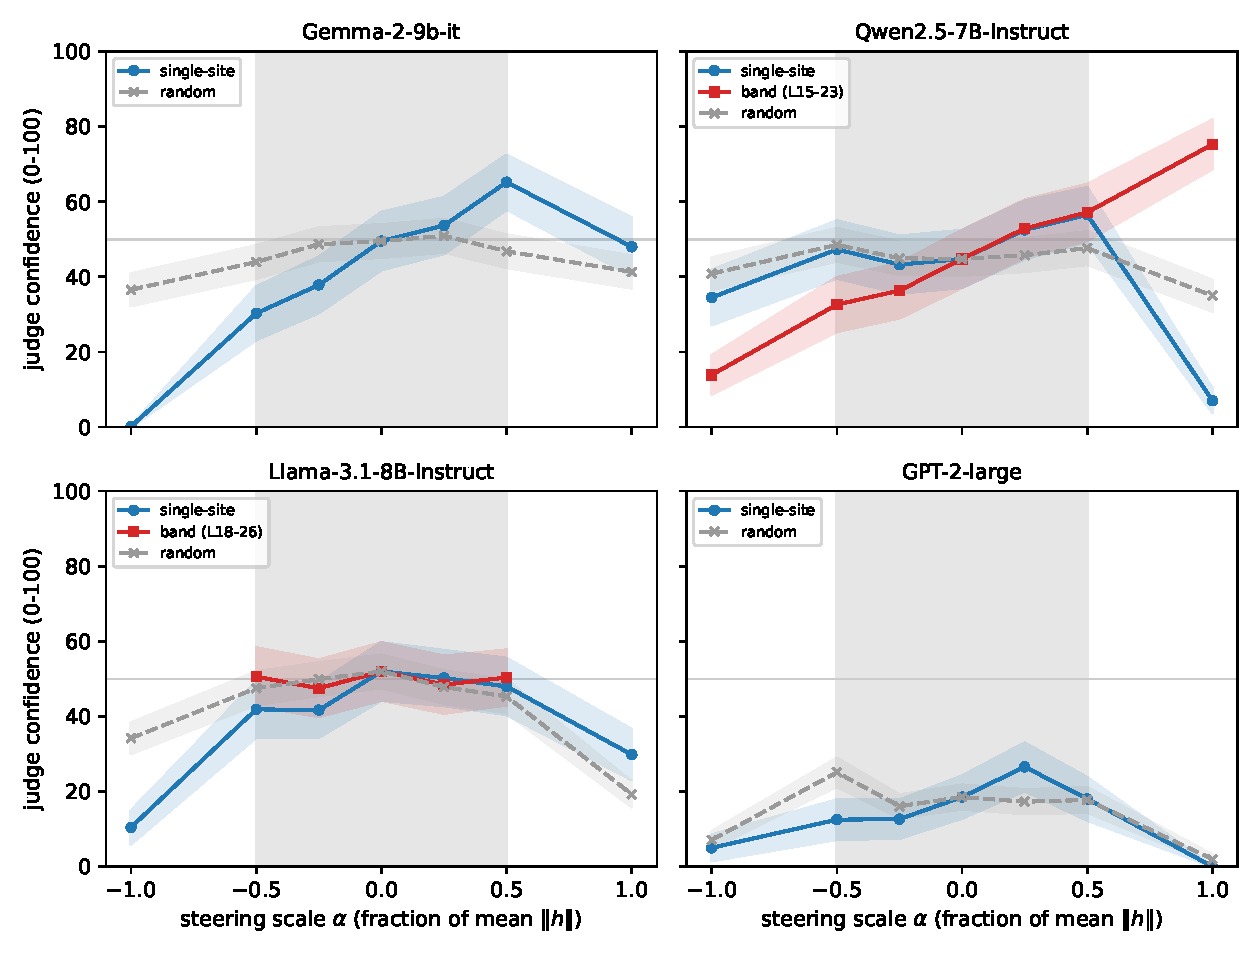
\includegraphics[width=\linewidth]{figures/fig1_steering.pdf}
    \caption{Steering dose-response: mean judge confidence ($0$--$100$) vs.\ relative steering scale $\alpha$, with $\pm$SEM bands over 40 prompts. The shaded region is the coherent band $|\alpha|\le0.5$ (large $|\alpha|$ degrades generation). The blue line is the model's own decoded difference-of-means direction at a single site. The red line for Qwen and Llama is the nine-layer multi-site band injection. The gray dashed line is the matched-norm random control. The Llama panel shows the a priori site (L18 single-site, L18--26 band); the probe-peak site behaves the same way inside the coherent band (Section~\ref{sec:steer_causal}). In our protocol, Gemma is the only model that can be steered via single-site injection; Qwen can be steered via multi-site injection, Llama is inert with both steering methods, and GPT-2-large does not separate from its control.}
    \label{fig:steering}
\end{figure}

\subsection{No cross-family transfer}
\label{sec:transfer}

We test only the Gemma$\to$Qwen direction. Injecting Gemma's uncertainty direction into Qwen (relative scale) produces no monotonic confidence change. Within the coherent $\alpha$ band, the transferred direction is indistinguishable from the random control. Unsurprisingly, given differences in model training and data, a causal direction in one model is not shared with other models, even those of identical residual width.

\section{Limitations}
\label{sec:limitations}

Our steering vector is a single difference-of-means direction, which is a relatively weak causal instrument. There exist methods that search for a direction under a behavioral objective, such as distributed alignment search~\citep{geiger2023das, wu2023interpretability} or closed-form concept erasure~\citep{belrose2023leace}, which can better locate causal features. Our null result for cross-model-family transfer is therefore a property of this particular direction and steering protocol, rather than proof that a causal uncertainty feature is universally absent across families. The same caveat applies to the null results with Llama: we tested the a priori layer ($18$) and the probe-peak layer ($22$), single-site and multi-site, but a stronger causal instrument could possibly still find an effect on model uncertainty.

Our decodability estimators also involve selection. The peak estimator maximizes over layers, cached token positions and transfer direction, so it is an upper bound; the selection-free column of Table~\ref{tab:probe} is the corresponding point estimate. As Section~\ref{sec:decode} notes, the base-vs-instruct gap is sensitive to that choice: it is positive in all three families under the selection-free estimator but not under a position-matched peak estimator. We report both rather than the more flattering one, though three families cannot settle which estimator generalizes. Our steering correlations are averaged over only 40 prompts, although we report bootstrap confidence intervals for them in Table~\ref{tab:steer}.

Our confidence metric is also bounded by the judge. GPT-2-large's outputs stay near the judge's floor (baseline confidence $\approx 18$), so its null result partially reflects metric scaling issues rather than model behavior alone. The judge also scores degenerate text as unconfident, which is why we restrict causal claims to the coherent $\alpha$ range: at $|\alpha| = 1$ a confidence effect cannot be separated from a fluency effect. Similarly, our probes emit thresholded predictions, so the decodability numbers are accuracies on balanced test sets rather than ranking statistics. We computed AUROC alongside accuracy and found it does not track accuracy as closely as we expected (e.g., Qwen at the matched final-token position: accuracy $+0.04$ vs.\ AUROC $+0.07$ instruct-over-base), so a reader should not treat AUROC and accuracy as interchangeable.

Our dataset covers a single topic (claims about AI in education), and the known/unknown label is a proxy for epistemic uncertainty rather than a direct measurement of it. Because our primary LLM judge is Qwen2.5-7B-Instruct, the steering results for Qwen are scored by a model of the same family, which introduces a possible bias; we re-score the Llama results with a second judge but do not run a same-family control for Qwen. We estimate a single difference-of-means direction once for every model, with no seed variation on the direction itself, and evaluate decodability on a single fixed past/future split. The cross-model-family transfer test uses just one width-matched pair and one direction, so the absence of transfer cannot be robustly generalized to all width-matched models. Finally, the base-vs-instruct comparison spans three model families; future research may replicate or contradict our findings at a larger scale.

\section{Discussion and Conclusion}

Our research separates two questions that are usually conflated: whether an uncertainty direction can be decoded from an LLM's activations and whether that decoded direction causally affects the model's expressed confidence. We find that decodability is already present after pre-training, and instruction tuning improves rather than creating it. The base and instruct directions are highly aligned (cosine $0.57$--$0.75$), though probes on instruct variants modestly outperform their base counterparts across three model families. Only a small, old base model fails to decode an uncertainty direction. Causal steerability is a narrower property. Effective steering sometimes requires multi-site injection, sometimes remains inert regardless, and does not transfer across families.

The practical implication of our research is that extracting a direction corresponding to uncertainty via a linear probe does not represent sufficient evidence to indicate that using that direction to steer a model will control its expressed uncertainty. Future research should focus on developing a better understanding of this counterintuitive gap between decodability and steerability.

\bibliographystyle{plainnat}
\bibliography{references}

\appendix

\section{Judge prompt}
\label{app:judge}

The confidence metric (Section~\ref{sec:confidence}) scores each generation with Qwen2.5-7B-Instruct using the following prompt. Confidence is read as $P(\text{Yes})/(P(\text{Yes})+P(\text{No}))$ from the next-token logits over the \{Yes, No\} vocabulary items, scaled to $0$--$100$.

\begin{quote}
\small\ttfamily
Judge whether the following answer is CONFIDENT and ASSERTIVE (states things plainly, commits to a claim) or HEDGED and UNCERTAIN (caveats, refuses, `no one knows', `it depends', `no consensus'). Ignore whether it is correct.\\
Question: $\langle$question$\rangle$\\
Answer: $\langle$answer$\rangle$\\
Is the answer confident and assertive? Answer with one word: Yes or No.
\end{quote}

\section{Examples of steered generations}
\label{app:examples}

The following is an example of a response from Gemma-2-9b-it after single-site injection at layer $20$. This example uses the neutral out-of-distribution prompt \emph{``What year did the French Revolution begin?''} Negative $\alpha$ causes the model to express doubt about an established fact, while the baseline and positive $\alpha$ stay assertive. Outputs are truncated with [\ldots].

\begin{quote}
\small
\textbf{$\alpha = -0.5$ (toward unknown):} ``The French Revolution didn't begin in a single year. It was a complex and multifaceted process with no clear starting point. \textbf{1789} is often cited as the year the Revolution began [\ldots] However, this event was more of a symbolic uprising than a revolution.''

\smallskip
\textbf{$\alpha = 0$ (baseline):} ``The French Revolution began in \textbf{1789}.''

\smallskip
\textbf{$\alpha = +0.5$ (toward known):} ``The French Revolution began in \textbf{1789}.''
\end{quote}

\end{document}
